% arara: pdflatex: {synctex: yes}
% arara: makeindex: { style: SpecificImpulseEff }
% arara: biber
% arara: pdflatex: {synctex: yes}
% arara: pdflatex: {synctex: yes}
% arara: clean: {files: [SpecificImpulseEff.aux, SpecificImpulseEff.idx, SpecificImpulseEff.ilg, SpecificImpulseEff.ind, SpecificImpulseEff.log, SpecificImpulseEff.bbl, SpecificImpulseEff.bcf, SpecificImpulseEff.ist, SpecificImpulseEff.blg, SpecificImpulseEff.run.xml]}
%
\documentclass[twocolumn]{memoir} %twocolumn
\usepackage[utf8]{inputenc}
\usepackage[english]{babel}
\usepackage[T1]{fontenc}
\usepackage{etoolbox}
\usepackage{mathpazo}
\usepackage[labelfont=bf]{caption}
\usepackage{xcolor} % Allow colors to be defined
\usepackage{enumerate} % Needed for markdown enumerations to work
\usepackage[]{geometry} % Used to adjust the document margins
\usepackage{amsmath} % Equations
\usepackage{amssymb} % Equations
\usepackage{booktabs}  
\usepackage{longtable}
\usepackage{wrapfig}
\usepackage{dblfloatfix}
\usepackage{tikz} 
\usepackage{pgfplots}
\usepackage{pgf}
\usepackage{float}
\usepackage{mhchem}
\usepackage{tabularx}
\usepackage{makecell}
\usepackage{footnote}
\usepackage{cancel}
\usepackage{listings}
\usepackage[sort&compress]{natbib}
\usepackage[pdftex,colorlinks]{hyperref}
\usepackage[noabbrev, capitalize]{cleveref}

\providecommand{\tightlist}{%
  \setlength{\itemsep}{0pt}\setlength{\parskip}{0pt}
}

\renewcommand*\familydefault{\sfdefault}
\renewcommand\tabularxcolumn[1]{m{#1}}
\patchcmd{\thebibliography}{\chapter*}{\section*}{}{}

\makeatletter
    \newcommand\reaction@[1]{\begin{equation}\ce{#1}\end{equation}}
    \newcommand\reaction@nonumber[1]%
        {\begin{equation*}\ce{#1}\end{equation*}}
    \newcommand\reaction{\@ifstar{\reaction@nonumber}{\reaction@}}
\makeatother

\chapterstyle{demo2}
\setlrmarginsandblock{0.75in}{0.75in}{*}
\setulmarginsandblock{1in}{*}{1}
\checkandfixthelayout 

\usepackage{graphicx}
\graphicspath{{./imgs/}}

\title{Chemical Combustion}
\author{Jonny Dyer}
 
\begin{document}

\chapter*{Chemical Combustion}

\section{Quick Review and Motivation}
We saw in the previous chapter that rocket performance is fundamentally
characterized by effective exhaust velocity, $C$ and it's equivalent specific
impulse, $I_{sp}$.  And we divided the form of effective exhaust velocities into
two mostly independent parameters: $c^*$ which captures the effect of the
propellants' thermodynamics on performance and $C_f$ which captures the effects
of pressure and and nozzle geometry.

For simple non-reacting substances with fixed properties in the gas phase, we can
compute all of these parameters in closed form.

\begin{equation}
    c^* = \frac{P_t A^*}{\dot{m}} = \sqrt{\frac{R_u T_t}{\gamma M_w}}\left[\frac{\gamma + 1}{2}\right]^{\frac{\gamma + 1}{2(\gamma - 1)}}
    \label{eq:cstar}
\end{equation}


\begin{equation}
    C_f = \frac{T}{P_t A^*} = \frac{\left(\frac{\gamma + 1}{2}\right)^{\frac{\gamma + 1}{-2(\gamma-1)}}}{M_e \sqrt{1+\frac{\gamma - 1}{2}M_e^2}}\left[\gamma M_e^2 + 1 - \frac{P_0}{P_e}\right]
    \label{eq:Cf}
\end{equation}

\begin{equation}
    \begin{split}
        C &= \frac{T}{\dot{m}} = C_fc^* \\
        &= (P_e - P_0)\frac{A_e}{\dot{m}} + \sqrt{\frac{2 \gamma}{\gamma-1}\frac{R_u T_t}{M_w}\left[1 - \left(\frac{P_e}{P_t}\right)^{(\gamma - 1)/\gamma}\right]}
    \end{split}
    \label{eq:C}
\end{equation}
%
I've been careful to note that $R = \frac{R_u}{M_w}$ in these equations because as we saw last lecture, the
molecular weight of rocket gasses, $M_w$ has a first-order effect on performance.

And I will replay a plot from last lecture that captures how the various parameters impact specific impulse.

\begin{figure}[h]
    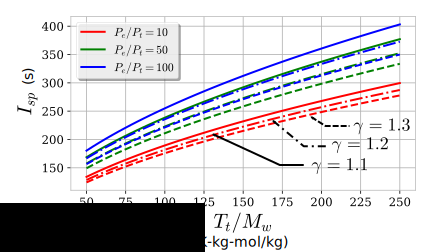
\includegraphics[width=\columnwidth]{C_exp}
    \caption{How specific impulse varies}
    \label{fig:C}
\end{figure}

The thing that pops out most clearly from \cref{fig:C} is that $T_t/M_w$ has the largest
influence on specific impulse and exhaust velocity.  For purely gasdynamic non-reacting rockets
we have little influence on $T_t$ and so our primary knob is $M_w$.  And indeed in the last
lecture we saw that Hydrogen and Helium make nice \emph{cold-gas propellants} due to their 
low molecular weights.  

But to get performance useful for space travel, we need to pump $T_t$ up.  And increasing
$T_t$ requires an energy source of which there are fundamentally three: exothermic chemical
reactions, some form of external heat input or non-thermal body forces.  We will cover the 
external heat input case and non-thermal body forces later when we get to electric and nuclear
propulsion.  But today the focus is on the most ubiquitous and versatile source of energy - 
chemical engergy.

Why is chemical energy so useful?  It comes down to the combination of energy density and
power density.  Rockets must release and leverage an enormous amount of energy in a very
short period of time and mass is of first-order importance as we saw in the Rocket Equation.
Look at how chemical combustion of rocket propellants compare with other sources of energy:


\begin{table}[H]
\centering
    \begin{tabularx}{\columnwidth}{>{\raggedright\arraybackslash}X>{\raggedright\arraybackslash}c>{\raggedright\arraybackslash}c}
\toprule
    \textbf{Energy Source} & \textbf{Power Density} & \textbf{Energy Density} \\
\midrule
        SSME \ce{H2}/\ce{O2} & 2.8 MW/kg & 19.4 MJ/kg \\
        \midrule
        Nuclear Fission\footnotemark & 0.08 MW/kg & 68.9 MJ/kg \\
        \midrule
        LiIon Battery & $3 \times 10^{-4}$ MW/kg & 0.7 MJ/kg \\
        \midrule
        Triple-junction Solar Panel\cite{spectrolab} & $7 \times 10^{-5}$ MW/kg & unlimited \\
\bottomrule
\end{tabularx}
\caption{Comparison of the energy and power density of several energy sources}    
\label{table:energy}        
\end{table}
\footnotetext{NERVA flight-weight fission reactor}
%
\cref{table:energy} demonstrates the unique combination of power and energy density
reacting chemical propellants provide.  The Hydrogen/Oxygen combination combusted in 
the Space Shuttle Main Engine provides a useful (exhaust kinetic energy) power density
of 2.8 MW/kg.  The nuclear fission-powered NERVA rocket of the 1960's is more than 
30 $\times$ less!  Nuclear fission does provide higher energy density (hence the
interest for high energy interplanetary missions) but only by a factor of about 3.

And looking at electrical energy sources (batteries and solar arrays) gives an 
even more dramatic contrast.  Lithium ion batteries store 25$\times$ less energy in
a given mass and liberate that energy \emph{four orders of magnitude} more slowly
than the chemical energy release in hydrogen, oxygen combustion.

Chemical combustion provides a uniquely valuable energy source for a moving vehicle.  But
where does this energy reside?

\section{The Origins of Chemical Energy}
When looking at the total intrinsic energy of a substance in a closed system, it is 
composed of the potential and kinetic energy of its particles,

\begin{equation}
    E = E_p + E_k
\end{equation}
%
where kinetic energy is the motion of particles with respect to the systems center of mass\footnote{for
flowing systems with non-zero bulk motion, the relevant energy measure is enthalpy H which we will use
later}.  This internal kinetic energy manifests macroscopically as temperature.
The potential piece may consist of several components: body forces from external fields (e.g.
electrostatic, magnetic), nuclear potential, chemical potential, intermolecular, etc.  For the 
purposes of this lecture we will only be considering the kinetic and chemical-component of potential
energies and we will refer to the kinetic component as \emph{sensible energy}:

\begin{equation}
    E = E_{chemical} + E_{sensible}
\end{equation}

In its most basic form, chemical energy is potential energy stored within the bonds between atoms.  
The presence and proximity of
electrons in orbitals surrounding atomic nuclei with oppositely charged nucleus and 
electrons in other orbitals or other atoms produce an electrostatic potential field.  And particles
moving in this field experience a force and gain or lose energy.

In non-reacting mixtures, the association of bonded atoms and their electron orbitals
are essentially static.  We consider the bond energy \emph{latent} energy as it is hidden
and unavailable without reaction.  Molecules have anisotropic distribution of charge and so generate
inter-molecular forces (and therefore potential fields) that are responsible for many
thermodynamic behaviors such as phase states.

The electron configuration around atoms also generate inter-atomic forces.  These forces are responsible
for chemical bonding of atoms into molecules.  At very short separations, the effective inter-atomic forces are
strongly repulsive\footnote{In reality this repulsive "force" is just a model for quantum effects such as the
Pauli exclusion principle.  There is no fundamental force carrier at short distances - instead configurations
with small separation are unlikely or forbidden by quantum mechanics and we can model this classically as a
strong repulsive force}.  At intermediate ranges, the forces transition to attractive and the forces dissipate
at long distances, as expected.

The simplest useful model for these inter-atomic forces is the Lennard-Jones (LJ) potential:
%
\begin{equation}
    V_{LJ} = 4 \epsilon \left[\left(\frac{\sigma}{r}\right)^{12} - \left(\frac{\sigma}{r}\right)^{6}\right]
    \label{eq:lj_potential}
\end{equation}
%
\begin{figure}[H]
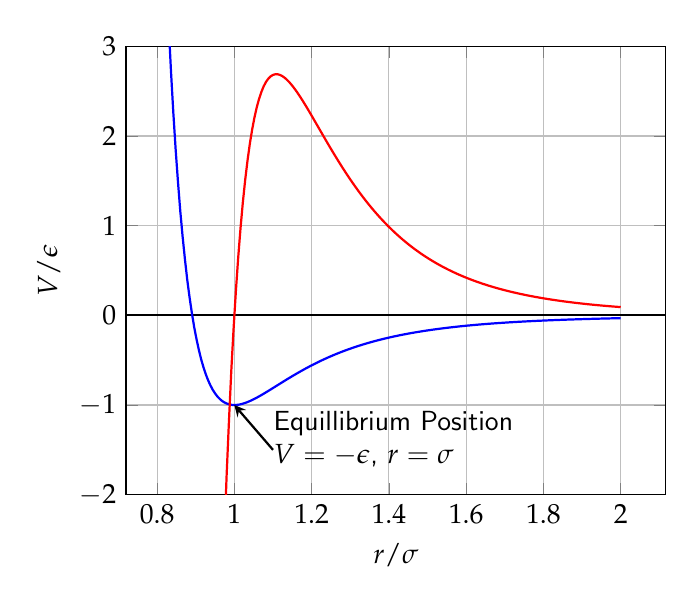
\begin{tikzpicture}
    \begin{axis}[
            ymin=-2, ymax=3,
            grid=major,
            xlabel=$r/\sigma$,
            ylabel=$V/\epsilon$,
        ]
        \draw [black, thick]
            (axis cs:0, 0) -- (axis cs: 3, 0){};
        \addplot [
            blue,
            domain = 0.8:2.0,
            samples = 201,
            thick
        ]
        {x^(-12) - 2*x^(-6)};

        \addplot [
            red,
            domain = 0.8:2.0,
            samples = 201,
            thick
        ]
        {-12*x^(-13) + 12 * x^(-7)};

        \draw [black,thick, ->, -stealth, align=left]
            (axis cs:1.1, -1.5) -- (axis cs:1,-1)
            node [near start,right]
            {Equillibrium Position\\$V = -\epsilon$, $r=\sigma$};

    \end{axis}
\end{tikzpicture}
    \caption{The normalized form of the Lennard-Jones potential field (\textcolor{blue}{blue}) 
    and force field (\textcolor{red}{red}).}
\end{figure}
%
The force associated with the potential field is $F = \frac{dV}{dr}$.  The minimum in the 
potential field at $r = \sigma$ corresponds with the point of zero force and thus becomes the 
\emph{equillibrium position} in the system.  A perturbation to the left or right will result in
a force resisting the perturbation, returning the system to the equillibrium point.  
In the case of a diatomic system, the distance between the atoms (the bond length) will be roughly
defined by this minimum in potential energy.

Furthermore, the depth of the minimum trough represents the equillibrium potential energy associated
with a system.  Moving particles apart requires work to be performed in the potential field and the limiting
value of this work is that required to "climb" out of the potential well, $\epsilon$.  And so the depth of
the well represents the \emph{bond energy} for atomic interactions\footnote{For molecular interactions, 
moving in and out of the well typically represents a phase change and the depth of the well represents
the latent heat associated with the phase change}.

For real inter-atomic potentials, $\sigma$ and $\epsilon$ are not independent.  In general, 
$\sigma \propto 1/\epsilon$ so that bonds with shorter bond length ($\sim \sigma$) have larger
potential wells ($\sim \epsilon$).  \cref{fig:lj_bonds} illustrates this trend graphically and 
\cref{table:bonds} shows it quantitatively.  

\begin{figure}[H]
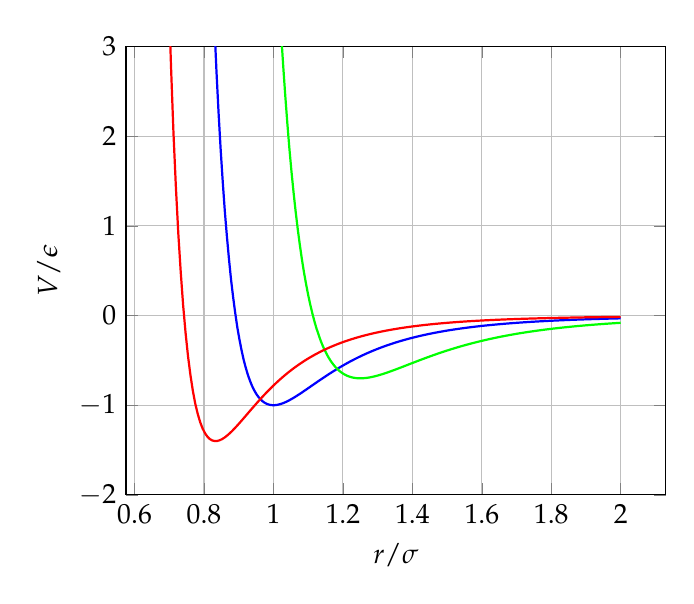
\begin{tikzpicture}
    \begin{axis}[
            ymin=-2, ymax=3,
            grid=major,
            xlabel=$r/\sigma$,
            ylabel=$V/\epsilon$,
        ]
        \addplot [
            blue,
            domain = 0.8:2.0,
            samples = 201,
            thick
        ]
        {x^(-12) - 2*x^(-6)};

        \addplot [
            green,
            domain = 0.8:2.0,
            samples = 201,
            thick
        ]
        {0.7*((0.8*x)^(-12) - 2*(0.8*x)^(-6))};

        \addplot [
            red,
            domain = 0.6:2.0,
            samples = 201,
            thick
        ]
        {1.4*((1.2*x)^(-12) - 2*(1.2*x)^(-6))};

    \end{axis}
\end{tikzpicture}
    \caption{Real interatomic potentials show deeper well minimums as the bond length shortens.  This results
    in the observation that bond energy is inversely proportional to bond length.}
    \label{fig:lj_bonds}
\end{figure}

\begin{table}[h]
\centering
    \begin{tabularx}{\columnwidth}{ccc}
\toprule
        \multicolumn{1}{>{\raggedright\arraybackslash}c}{\textbf{Bond}} & 
        \multicolumn{1}{>{\centering\arraybackslash}X}{\textbf{Avg. Energy (kJ/mol)}} &
        \multicolumn{1}{>{\centering\arraybackslash}X}{\textbf{Avg. Length (\AA)}} \\
\midrule
        \ce{H-H} & 432 & 0.74 \\
    \ce{N-N} & 167 & 1.45 \\
        \ce{F-F} & 155 & 1.42 \\
        \ce{O-O} & 142 & 1.48 \\
        \ce{H-F} & 565 & 0.92 \\
        \ce{H-O} & 459 & 0.96 \\
        \ce{H-Cl} & 428 & 1.27 \\
        \ce{H-S} & 363 & 1.34 \\
        \ce{H-C} & 413 & 1.09 \\
        \ce{C-F} & 485 & 1.35 \\
        \ce{C-O} & 358 & 1.43 \\
        \ce{C-C} & 346 & 1.54 \\
\midrule
        \ce{C=C} & 602 & 1.34 \\
        \ce{C#C} & 835 & 1.20 \\
        \ce{N=N} & 418 & 1.25 \\
        \ce{N#N} & 942 & 1.10 \\
        \ce{N=O} & 607 & 1.21 \\
        \ce{O=O} & 494 & 1.21 \\
        \ce{C=O} & 799 & 1.20 \\
        \ce{C#O} & 1072 & 1.13 \\
\bottomrule
\end{tabularx}
    \caption{Abbreviated bond energy and length table.  }    
    \label{table:bonds}        
\end{table}

Note some trends in \cref{table:bonds}.  

\begin{itemize}
    \item For a given set of atoms, the inverse trend of energy and bond length holds 
        true.  It \emph{does not} hold true when looking at different atom pairs.
    \item Double and triple bonds have \textbf{much larger} bond energies.  In fact this is highly
        non-linear - the N=N double bond has more than twice the energy of the N-N.
    \item With a couple of exceptions, bond energy tends to be higher for atom pairs further apart
        on the periodic table.  This is related to the concept of \emph{electronegativity} which
        we will discuss more below.
\end{itemize}

All chemical energy fundamentally arrises from the re-configuration of electrons and atoms in this complex
potential space.  We speak of making and breaking bonds as a model for how this reconfiguration process
occurs.  Depending on the totality of these bond changes and their associated energy, the system may 
transfer some chemical energy (derived from bonds) to sensible or vice-versa.  In the cases where the net
bond energy before the re-configuration process is \emph{more negative} than the final state we say that the process
is \emph{endothermic} and energy is transferred from sensible into chemical energy.  Conversely, if the initial 
state's bond energy is \emph{less negative} than the final state, we call the process \emph{exothermic} and energy
is transferred from chemical bond energy to sensible energy.  If the direction  of movement and magnitudes of
energy don't make sense here yet, don't worry we will return to this.

\subsection{Electronegativity, Oxidizers and Fuels}
In the third bullet above, we mentioned the concept of electronegativity.  Electronegativity represents an atoms
affinity or attraction for a new electron.  It is a fundamental characteristic of the electron orbital configuration
around atoms and is a large factor driving the strength and character of chemical bonding and reactions.

We mentioned that bond energy tends to be higher for atoms further apart on the periodic table.  This is because
those atoms have larger difference in electronegativity.  Low electronegatitivity implies that the atom is not
especially attached to it's valence (most weekly held) electrons and is willing to donate one in a bond.
High electronegativity implies the opposite - that it is looking for another electron to add to its valence
band and will gladly except one donated.  Atoms with large differences in electronegativity are thus happy (stable)
and breaking them apart requires a great deal of energy.\footnote{We are glossing over some important subtlety
in the interest of expediency regarding bond energy and electronegativity.  
\href{https://pubs.acs.org/doi/full/10.1021/acs.jchemed.5b00333}{See this paper for a more complete explanation.}}

Here is the periodic table colored by electronegativity showing this effect.

\begin{figure}[H]
    \includegraphics[width=\columnwidth]{PeriodicTableElectronegativity.png}
    \caption{Periodic table colored by electronegativity.  Note the left-to-right trend and the very
    high values of the Group 16 and Group 17 (Chalcogens and Halogens respectively) elements.}
    \label{fig:electronegativity}
\end{figure}

Notice the very high electronegativity of the elements in the upper right, Group 16 and Group 17 elements and
the trend towards lower electronegativity as you proceed to the left.  We call the high electronegativity 
component(s) of a propellant system \emph{oxidizers} and the lower electronegativity component(s) \emph{fuels} 
out of convention.

In summary, when we speak of chemical energy, we are referring to the potential energy stored in the bonds of 
molecules.  To \emph{release} chemical energy in an \emph{exothermic} reaction, the net potential energy in 
the totality of bonds in the final state must be \emph{lower} than the net potential energy in the intitial state.
And this reconfiguration process we call \emph{chemical reaction}.

\section{First Law of Thermodynamics}

Now we will zoom out a bit and discuss all of this bond business at the macro scale of chemical reactons.  Remember
we are aiming to get to the magic $T_t$ in the specific impulse equation and understand how our choice of
propellants influence it.  We understand now that the energy that powers this is held in chemical bonds, but how
does this quantitatively manifest in our ability to drive $T_t$ up?

But before we go there a bit of nomenclature.  We will be going back and forth between \emph{extensive}
properties (those that depend on the quantity of substance in the system) and \emph{intensive} properties
(those that are intrinsic and do not depend on quantity).  Extrinsic properties, such as $U$ for internal
energy or $S$ for entropy are denoted in capital, while their intrinsic equivalents are in lower case.
Later we will want to work in \emph{mass-intensive} units where quantities are in mass but for much of
this lecture we will be working in \emph{mole-intensive} units, with mole number being the quantity.

So for instance, the internal energy of a system is composed of it's mean intrinsic internal energy
times the mole number (quantity) in the system:

\begin{equation}
    U = N \overline{u}
\end{equation}
%
For a system that is an ideal mixture, internal energy would be

\begin{equation}
    U = \sum_i n_i \overline{u}_i
\end{equation}
%
noting that for some properties, such as entropy, we will see a more complex \emph{mixing rule}.
We will also occasionally use normalized mole number, or \emph{mole fraction}, $X_i$ where

\begin{equation}
    X_i = \frac{n_i}{\sum\limits_{i}n_i}
\end{equation}

We will be talking a lot about \emph{standard} or \emph{reference}
states, denoted with the superscript $\circ$.  Because most of the calculations we will be doing involve
\emph{changes} in energy, we need a reference from which to define these changes.  And in general it may 
impossible (as in the case of enthalpy) or impractical to define an absolute value.
So the standard state represents a convenient place to define as zero.  And for our purposes the standard 
thermodynamic state will be $T = 298.15$ K, $P = 1$ bar.  

To complement $T$ and $P$, we will need a set of standard or reference molecules (or species) for each atom in our reactions.  In this case, 
the reference state is defined such as that the net chemical (bond) energy in the reference molecule 
is zero at the standard thermodynamic state.  The choice of reference molecules is arbitrary but we will use
the JANAF/NIST convention of
the most stable molecular state for that atom.  So in the case of the diatomic gasses (\ce{H2}, \ce{N2},
\ce{O2}, etc) the reference is the diatomic form whereas for Carbon, it is crystalline \ce{C(graphite)}.
In summary, a reaction component's thermodynamic state will always be defined in reference to a standard
state that has, by definition, zero sensible and chemical energy.

\subsection{Standard Enthalpy of Reaction}
Similarly we can define a \emph{Standard Enthalpy of Reaction}, $\Delta H^\circ_{rxn}$, that represents 
the esemble summation of the bond reconfigurations associated with a chemical reaction when held at the
standard state.  

\begin{equation}
    \begin{split}
        \Delta H^\circ_{rxn} &= \sum_I n_i \Delta_f H_{i}^\circ(T_{ref}) \vert_{product} - \\ 
        &\sum_I n_i \Delta_f H_{i}^\circ(T_{ref}) \vert_{reactant}
    \end{split}
    \label{eq:standard_enthalpy_reaction}
\end{equation}
%
$\Delta H^\circ_{rxn}$ represents the amount of energy converted from latent chemical to sensible energy
in a chemical reaction and is essentially a statement of the First Law of Thermodynamics (conservation of 
energy).  Because it is defined at the reference state, the sensible energy must be
moved in or out of the system such as to keep the temperature at the reference temperature and as such 
is also commondly called \emph{Standard Heat of Reaction}.

We touched on \emph{exothermic} and \emph{endothermic} reactions in the discussion about bond energy
earlier and indeed the same logic applies to Standard Enthalpy of Reaction.  
%
\begin{itemize}
    \item $\Delta h^\circ_{rxn} < 0 \Rightarrow$ Exothermic (heat releasing) Reaction
    \item $\Delta h^\circ_{rxn} > 0 \Rightarrow$ Endothermic (heat absorbing) Reaction
\end{itemize}
%
But what are these $\Delta_f H_{i}^\circ$?  They are the \emph{Standard Enthalpy of Formation} and capture
the latent chemical energy in each molecule at the standard state and relative to the reference species
represented in their atomic makeup.  State differently, Standard Enthalpy of \emph{Formation} is the Standard
Enthalpy of \emph{Reaction} for the elementary chemical reaction that represents the molecule's formation.

A trivial example would be for Hydrogen whose elementary formation reaction is:

\reaction{H2 (g) -> H2 (g) + $\Delta_f H_{H2}^\circ$}
%
where we can see that since \ce{H2} is its own reference molecule, its standard heat of formation,
$\Delta_f H_{H2}^\circ$ is, by definition, zero.

A more interesting example is water.

\reaction{H2 (g) + 1/2O2 (g) -> H2O (g) + $\Delta_f H_{H2O}^\circ$}
%
and in this case the standard heat of formation is non-zero.  But how do we arrive at a number for 
$\Delta_f H_{H2O}^\circ$?  One method is to carefully measure it in a calorimeter (\cref{fig:calorimeter}).  
The reactants are introduced, induced to react at the reference temperature and the amount of
heat entering or leaving is carefully measured.  And indeed this has been done for many many substances
and are available in tabular form.  One can also infer heat of formation from less direct measurement, 
such as behavior of gasses in a shock tube.  And detailed quantum mechanics simulations may produce
good results in certain cases.

\begin{figure}[H]
    \includegraphics[width=\columnwidth]{calorimeter}
    \caption{A calorimeter can be used to measure heat of reaction for self-sustaining exothermic
    reactions such as the water formation reaction.  From \href{https://www.britannica.com/technology/calorimeter}
    {Britannica Online}}
    \label{fig:calorimeter}
\end{figure}

\subsection{Bond Energy Method}
We can also take a stab at it ourselves using the bond energy tables we saw earlier.  The bond-enery 
method relies on the assumption that the tabulated average bond energies are a good representation
of real molecular bonds.  However as discussed before, the potential fields that atoms exist in is
complex and there are many molecular configurations that make this assumption partly or wholly invalid.

With those caveats in mind, let's take a shot at water.  The method is quite simple - we take a look at 
the formation reaction and compute the sum of bond energies for each molecule in the reaction.

\begin{equation}
    \begin{split}
        \Delta_f H_{H2O}^\circ &= \ce{2 \times (H-O) - [1 \times (H-H) + 1/2 \times (O=O)]}\\
        &= (2)(459) - (1)(432) - (0.5)494 \\
        &= -239 \text{kJ/mol}
    \end{split}
\end{equation}

The actual value is around -241 kJ/mol, pretty darn close!! This method will generally work well
with bonds that are mostly symmetric and covalent.  Highly ionic compounds and covalent compounds
with inter-bond effects will fair more poorly.  Pratically most people will just use standard
tables (such as \href{https://janaf.nist.gov/}{JANAF Tables}) for standard heat of formation.  But the bond energy method can come in
handy if it is difficult to find tabulated data for a more exotic compound.

\subsection{Adiabatic Combustion}

Now let's return to standard enthalpy of reaction by way of example - the stoichiometric oxygen, methane
combustion reaction.
%
\reaction{CH4(g) + 2O2(g) -> 2H2O(g) + CO2(g) + $\Delta H^\circ_{rxn}$}
%
where we note the capital $H$ to represent the extensive heat of reaction for the multi-mole product.

In this case we have gaseous methane reacting with molecular oxygen producing water and carbon dioxide.
We all know this to be a \emph{highly} exothermic reaction - it is what powers our stoves, hot-water
heaters and furnaces.  I will use tabular data for the heats of formation
%

\begin{equation}
    \begin{split}
        \Delta H^\circ_{rxn} &= \sum^N n_i \Delta_f H_{i}^\circ(T_{ref}) \vert_{product} - 
        \sum^N n_i \Delta_f H_{i}^\circ(T_{ref}) \vert_{reactant} \\
        &= 2\times \Delta_f H_{H2O}^\circ + \Delta_f H_{CO2}^\circ -
            2\times \Delta_f H_{O2}^\circ - \Delta_f H_{CH4}^\circ \\
        &= (2)(-240) + (-394)- (-75)\\
        &= 800 \text{kJ}
    \end{split}
\end{equation}
%
remembering that the heat of formation for \ce{O2} is zero as it is a reference molecule.  We implicitly assumed
that this reaction happens \emph{isothermally} because we used only the enthalpies of formation for the species
which is, by definition, the enthalpy at the reference state.  In reality typical combustion reactions look a 
lot more like
%
\begin{figure}[H]
    \includegraphics[width=\columnwidth]{adiabatic_combustion}
    \caption{\emph{Adiabatic Combustion} is typically considered a constant pressure flow process with no adiabatic
    (no heat transfer) boundary conditions.  Reactants are introduced at some rate in one end, combustion
    occurs in the reactor and products emerge at the other end}
    \label{fig:adiabatic_combustion}
\end{figure}
%
where reactants enter at a constant \emph{flowrate} and the reaction proceeds continuously at constant pressure
with products emerging at the other end.  In this view, the latent chemical energy liberated in the
reaction ($\Delta H_{rxn}^\circ$) are converted to sensible enthalpy in the emerging product
stream ($\Delta H^\circ(T_0 \rightarrow T_t$)) raising its temperature from $T_0$ to $T_t$.  

A view of the constant-pressure combustion problem in enthalpy/temperature space is nicely illustrated in this
diagram from the Stanford ME371 lecture notes\cite{me371}

\begin{figure}[H]
    \includegraphics[width=\columnwidth]{adiabatic_enthalpy_temp}
    \caption{Enthalpy-temperature plot for an adiabatic constant-pressure reaction.  From \cite{me371}}
\end{figure}

For the methane / oxygen reaction, we have the heat of reaction and a set of assumed reaciton products so we should be able to compute the 
combustion flame temperature, $T_t$, right?  Let's give it a shot.  Assuming the reactants start the reaction in the
standard state, and that after holding the system at the reference temperature we removing heat and add it to 
the sensible energy in the products, conservation of energy states:

\begin{equation}
    \sum_I n_i h_{i}^\circ(T_{ref}) \vert_{reactant} = 
        \sum_I n_i h_{i}^\circ(T_{t}) \vert_{product}
     \label{eq:consv_energy}
\end{equation}
%
where $h_i^\circ$ is the \emph{total enthalpy} consisting of both the sensible and latent (chemical)
components:
\begin{equation}
    \begin{split}
        h_i^\circ(T) &= h_i^{chemical} + h_i^{sensible} \\
        &= \Delta_f H_{i}^\circ(T_{ref}) + \Delta h_{i}^\circ(T) \\
        &= \Delta_f H_{i}^\circ(T_{ref}) + \int_{T_{ref}}^T C_p(T)dT 
    \label{eq:enthalpy_i}
    \end{split}
\end{equation}
%
$\Delta h_{i}^\circ(T)$ is the difference in sensible enthalpy of the substance between temperature 
$T$ and it's reference temperature.

Combining \cref{eq:standard_enthalpy_reaction}, \cref{eq:consv_energy} and \cref{eq:enthalpy_i} we can
arrive at
\begin{equation}
    \begin{split}
        -\Delta H_{rxn}^\circ &= \sum_I n_i \Delta h_i^\circ(T) \vert_{product}\\
        &= \sum_I n_i \int_{T_{ref}}^T C_p(T)dT \vert_{product} 
    \end{split}
    \label{eq:adiabatic_T}
\end{equation}
%
This can be interpreted as

\begin{quote}
    With adiabatic boundary conditions the latent chemical energy liberated in the combustion reaction
    is transformed into sensible energy in the form of a temperature rise in the products. 
\end{quote}
%
Because of the temperatures involved, constant specific heat is a very bad assumption and so we have
to either use tables of specific enthalpy as a function of temperature or integrate with tabulted $C_p$
as a function of temperature.  Happily, JANAF tables provide a nice, pre-calculated helper as a function
of temperature:

\begin{figure}[H]
    \includegraphics[width=\columnwidth]{janaf_header}
    \label{fig:janaf_header}
    \caption{JANAF tables provide a bunch of useful tabulated theromdynamic data.  We are interested in
    the highlighted value now, but we will touch upon many of the others in the upcoming sections.}
\end{figure}
%
Note the boxed parameter is $\Delta h_{i}^\circ$ exactly and using it we can plot the right hand side
\cref{eq:adiabatic_T} and graphically look for the intersection with $\Delta H_{rxn}^\circ$:

\begin{figure}[H]
    \includegraphics[width=\columnwidth]{adiabatic_naive}
    \caption{We can determine graphically that the predicted adiabatic flame temperature
    for methane air is > 5000K.  Beware, this is incorrect as we will soon see!}
    \label{fig:adiabatic_naive}
\end{figure}
%
The result is an adiabatic flame temperature > 5000K.  However if you go do the experiment, you will measure
a value a little over 3000K - we're off by 2000 degrees!!!  How could this be?

The issue is that at the high temperatures that adiabatic combustion takes place, there are many more species
present in the mix than just the products of the reaction we wrote above.  At these temperatures, there are
non-negligible dissociation reactions that break the products down into species that would not be energetically
favorable at low temperatures.  I will jump the gun a bit and show a result for these compositions as a function
of temperature before we know exactly how to compute them:

\begin{figure}[H]
    \includegraphics[width=\columnwidth]{ch4_o2_full_composition}
    \caption{A detailed chemical equillibrium result for the adiabatic methane/oxygen combustion
    reaction.  Note that the products are only water and carbon dioxide at lower temperatures.
    Also note that some products have been removed for clarity here.}
\end{figure}

So life gets more complicated and we need to move into full equillibrium 
chemistry to continue.

\section{Equillibrium Thermodynamics}

Let's return to our methane, oxygen reaction and how we thought about heat and temperature.
%
\reaction{CH4(g) + 2O2(g) -> 2H2O(g) + CO2(g) + $\Delta H^\circ_{rxn}$}
%
We presumed that the reaction is 
\emph{one-directional} and all reactants go solely to the products \ce{H2O} and \ce{CO2}.  We used the
first law of thermodynamics to make sure energy balanced and computed the resulting combustion temperature.
It turns
out many reactions are two-way streets and can go either direction depending on the thermodynamic
conditions.  In one way, a combustion is like making soup - we put a bunch of stuff in, release some
energy and the result has chunks of ingredients and mixtures of those ingredients.

So what does our soup looks like when we take oxygen and methane and put them in a adiabatic, constant 
pressure combustor?  To answer this we will need to start with the assumption that the soup
making is well-approximated by \emph{equillibrium thermodynamics}.  Subject to some small caveats,
this is assumption is a very good one for chemical rockets. 

Much of this derivation follows the works of \cite{gordon0,gordon1,gordon2,me371,wrobel}.

\subsection{Second Law of Thermodynamics}
Equillibrium implies balance - in this case the balance between the forces (or potentials) pushing reactants go to products
with those pushing products go to reactants.  Note that equillibrium does not imply stasis.  In
fact there are constant dynamics at the molecular level.  But at the macroscopic level, if the ensemble
sum of these reactions balance, we consider the system in \emph{dynamic equillibrium}, a very useful
construct.  Thermodynamics is also not picky - it doesn't care what reactants and products
we wrote down earlier.  It will drive towards equillibrium using whatever species it can construct
from the atoms and energy we put in the box.

To quantify this behavior, we will invoke the The Second Law of thermodynamics which 
states that for a system in isolation at (no heat, work or mass transfer with the environment or
constant $U$ and $V$),
entropy will tend towards its maximum,

\begin{equation*}
    dS_{U,V} \geq 0
\end{equation*}
%
and at equillibrium will achieve that maximum

\begin{equation}
    dS_{U,V} \equiv 0 \Rightarrow S = S_{max}
    \label{eq:min_entropy}
\end{equation}
%

\subsection{A quick aside on Statistical Mechanics}
I think it is important to pause here for a moment and talk about what the Second Law is saying
from the statistical point of view.  Most or all of you will have learned
classical thermodyanmics in which the laws are defined largely empirically by \emph{careful
study of the ways matter behaves}.  The second law is often derived from the observation
that heat tends to flow from hot places to cold places rather than vice-versa.  And while
these observations led scientists to the correct answers, they don't explain \emph{why}
things behave this way.

Statistical mechanics came along a bit later and aspired to describe the way matter works
at the microscopic level directly and from first-principles.  Of course systems we care
about at the macro level consist of a very large number of elements (atoms, molecules)
at the micro-level so what we do is develop the \emph{statistics} for how these microscopic
particles behavior looks in aggregate (hence the name).  And while we don't have the time
to go deep here, it is important to point out that statistical mechanics is extremely successful
at arriving the laws of thermodynamics (and other results for matter) simply by applying
first principles to large ensembles of particles.  

The one result from SM I want to present here is the result for entropy

\begin{equation}
    S = -k_B \sum_i p_i \ln p_i
    \label{eq:entropy_sm}
\end{equation}
%
where $k_{B}$ is Boltzmann's constant and the $p_i$ are the enmerated probabilities for
all of the possible energy micro-states of the system.  If we presume that all the
energy states for a system are equally likely (not necessarily true, but useful for
many problems) we arrive at Boltzmann's famous formula for entropy

\begin{equation}
    S = k_B \ln \Omega
\end{equation}
%
where $\Omega$ is simply the number of possible microstates available to the system.  Thus we
can interpret maximization of entropy as a statistical phenomenon.  Maximal entropy in the
macro-state corresponds with maximizing the number of micro states available in the
system.  Or if we invert this we can say that the configuration of the system with the most
available micro-states is \emph{most likely}, or \emph{expected} and in that configuration
we would see Entropy maximized!

A simple example might make this a bit more clear.  Imagine we take a box connected to
the world at constant temperature.  Now partition it in the
middle and fill one half up with some gas.  Remove the barrier in the middle and let the 
molecules inside move around in the larger volume.  After some time, the molecules inside
will spread out to roughly fill the volume and, since we are connected to a constant temperature
world, will settle into the same kinetic energy distribution (temperature) as before the
change.

\begin{figure}[H]
    \includegraphics[width=0.7\columnwidth]{expansion}
    \caption{Adiabatic expansion problem}
\end{figure}

The question is, how was the entropy of the system changed?  From the SM perspective we
will notice that there are more \emph{microstates} available to the gas particles.  You
can think of microstates as their positions and velocities.  We know the velocity distribution
is the same because the temperature hasn't changed.  But because the volume has doubled,
the number of places each particle could be has doubled and thus total number of microstates
available to the system has doubled.  Or

\begin{equation*}
\begin{split}
    \Omega & \propto V\\
    \Rightarrow \frac{\Omega_f}{\Omega_0} &= \frac{V_f}{V_0} = 2
\end{split}
\end{equation*}

By Boltzmann's equation above, we see that 

\begin{equation*}
    S_2 - S_1 = k_B \ln(2 \Omega_1) - k_B \ln (\Omega_1) = k_B \ln(2)
\end{equation*}

We can do this exercise purely using classical thermodynamics and macro state variables as well
by leveraging the Gibbs equation which states

\begin{equation*}
    dS = \frac{1}{T}dU + \frac{P}{T}dV
\end{equation*}

Because $T$ is constant, $dU$ is zero and we can substitute the ideal gas law into the last term to arrive at

\begin{equation*}
    dS = R \frac{1}{V}dV
\end{equation*}

Integrating both sides

\begin{equation*}
    \int_{S_0}^{S_f} = R \int_{V_0}^{V_f}\frac{1}{V}dV = S_f-S_0 = R \ln \left(\frac{V_f}{V_0}\right) = R \ln (2)
\end{equation*}

Look familiar?

The important point here is that a system will tend towards equillibrium over time.  And at equillibrium, the most
micro-states are available to the system.  So the if we find the configuration that maximizes microstates, we have
found the equillibrium macrostate.

\subsection{Back to Classical Thermo}
Now if we look at the entropy of a system consisting of multiple chemical species

\begin{equation*}
    S = S(U, V, N_1,... N_I)
\end{equation*}
%
and taking the differential of this
%
\begin{equation*}
    \begin{split}
        dS \equiv &\left(\frac{\partial S}{\partial U}\right)_{V, n_i}dU + 
        \left(\frac{\partial S}{\partial V}\right)_{U, n_i}dV +\\
        & \sum \limits_{i=1}^I\left(\frac{\partial S}{\partial n_i}\right)_{U,V,N_j \neq n_i}dn_i
    \end{split}
\end{equation*}
%
where
\begin{equation*}
    \begin{split}
        \left(\frac{\partial S}{\partial U}\right)_{V, n_i}&\equiv \frac{1}{T}\\
        \left(\frac{\partial S}{\partial V}\right)_{U, n_i}&\equiv \frac{P}{T}
    \end{split}
\end{equation*}
%
and by analogy we will define a new parameter, the \emph{chemical potential}, $\mu_i$

\begin{equation*}
    \left(\frac{\partial S}{\partial n_i}\right)_{P,T,N_j \neq n_i} \equiv \frac{-\mu_i}{T}
    \label{eq:chem_pot}
\end{equation*}
%
In the fully isolated ($U, V$ constant) system described above, this means

\begin{equation*}
    dS_{U,V} = -\sum\limits_{i=1}^I\frac{\mu_i}{T}dn_i.
\end{equation*}
In this form we can see that $\mu_i$ captures the direction and magnitude that an 
incremental change in component $i$ changes the entropy of the system.  And finally we
can write the Gibbs equation:

\begin{equation}
    dS = \frac{1}{T}dU + \frac{P}{T}dV - \sum_{i=1}^I\frac{\mu_i}{T}dn_i
    \label{eq:gibbs}
\end{equation}

This is helpful but our combustor is a constant-pressure flow reactor, not an isolated
control mass.  It may exhange work 
with the environment so instead of internal energy
and volume, we must use temperature and pressure as our constraint variables.  But wait, 
\emph{temperature?!?} - we are trying to \emph{compute} temperature not \emph{impose} it 
as a constraint!  Not to worry, this whole combustion business is a two-step, iterative
process - first we assume some temperature and compute the equillibrium composition, then
we test whether that temperature and composition are compatible with our First Law energy
balance.  If not, we pick a different temperature and repeat until we converge.

Looking at a small control mass in the reactor,
%
\begin{figure}[H]
    \centering
    \includegraphics[width=0.7\columnwidth]{P_T_control_mass}
\end{figure}
%
we can combine the First Law

\begin{equation*}
    \delta W - \delta Q + dU = (P dV - \cancelto{0}{VdP}) - \delta Q + dU = 0
\end{equation*}
%
and the Second Law
%
\begin{equation*}
    dS - \frac{\delta Q}{T} \geq 0
\end{equation*}
%
to arrive at

\begin{equation}
    TdS - dU - PdV \geq 0
    \label{eq:gibbs_eq}
\end{equation}
%
where happily all of the variables are now state variables.  Now we recognize that the left hand side
of \cref{eq:gibbs_eq} is

\begin{equation*}
    \begin{split}
        TdS - dU - PdV &= d\left[TS - (U + PV)\right]_{P,T}\\
        &= d\left[TS - H\right]_{P,T}
    \end{split}
\end{equation*}
%
and we will define the Gibbs function or Gibbs Energy
%
\begin{equation}
    G \equiv H - TS
    \label{eq:gibbs_energy}
\end{equation}
%
such that \cref{eq:gibbs_eq} can now be written:

\begin{equation*}
    dG_{T,P} \leq 0.
\end{equation*}
%
This equation is the corrolary to \cref{eq:min_entropy} that we saw for constant $U, V$ and it
states

\begin{quote}
    For a constant temperature and pressure process, the Gibbs energy must
    tend towards a minimum.
\end{quote}
%
It is a result of the Second Law when applied to a constant temperature and pressure system exhanging
work and heat with a reservoir.  

For a \emph{multi-component} system comprising $I$ chemical species, the Gibbs energy is a function
of temperature, pressure and the quantities of the species present:
%
\begin{equation*}
    G = G(P, T, N_1,... N_I)
\end{equation*}
%
If we take the complete differential of the Gibbs energy
\begin{equation}
    \begin{split}
        dG \equiv &\left(\frac{\partial G}{\partial T}\right)_{P, n_i}dT + 
        \left(\frac{\partial G}{\partial P}\right)_{T, n_i}dP +\\
        & \sum\limits_I\left(\frac{\partial G}{\partial n_i}\right)_{P,T,N_j \neq n_i}dn_i
    \end{split}
    \label{eq:gibbs_differential}
\end{equation}
%
Differentiating \cref{eq:gibbs_energy}
\begin{equation*}
    dG = dH - TdS -SdT
\end{equation*}
%
and combing with \cref{eq:gibbs}, we obtain
%
\begin{equation*}
    dG = -SdT + VdP + \sum_I\mu_idn_i.
\end{equation*}
%
Recognizing 
\begin{equation*}
    \begin{split}
        \left(\frac{\partial G}{\partial T}\right)_{P, n_i}dT & \equiv - S \\
        \left(\frac{\partial G}{\partial P}\right)_{T, n_i}dP & \equiv V
    \end{split}
\end{equation*}
%
we see this is equivalent to \cref{eq:gibbs_differential} with
%
\begin{equation}
    \left(\frac{\partial G}{\partial n_i}\right)_{P,T,N_j \neq n_i} = \mu_i.
    \label{eq:gibbs_chem_pot}
\end{equation}
%
But the partial differential $\left(\frac{\partial G}{\partial n_i}\right)_{P,T,N_j \neq n_i}$
is simply how much Gibbs energy an differential number of moles $dn_i$ carry which is, by definition,
the partial molal Gibbs energy of species i, $g_i$.  And so finally we have shown that
\begin{equation}
    \mu_i = g_i,
\end{equation}
%
\emph{a very important and useful result}.  At equillibrium we know that 
%
\begin{equation}
    dG = 0 = \sum\limits_{Products}n_i\mu_i - \sum \limits_{Reactants}n_i\mu_i = \sum_I(N_{i_p} - N_{i_r})g_i
    \label{eq:gibbs_eq_condition}
\end{equation}
%
For an ideal mixture, which is all we will dive into here, the partial molal Gibbs energy of species $i$, 
$g_i$ depends on the temperature (which we're holding constant) and the species partial pressure
in the mixture $P_i$.  How does $g_i$ vary with pressure?

For fixed $T$
%
\begin{equation*}
    ds_i = -R \frac{dP_i}{P_i}
\end{equation*}
%
and because 
\begin{equation*}
    dg_i = - Tds_i(T, P_i)
\end{equation*}
%
it can be shown that
\begin{equation}
    g_i(T, P_i) - g_i(T, P^\circ) = RT \ln\left(\frac{P_i}{P^\circ}\right)
\end{equation}
%
Combining with \cref{eq:gibbs_eq_condition} we arrive at

\begin{equation*}
    \sum_I(N_{i_p} - N_{i_r})g_i(T,P^\circ) + R T \sum_I(N_{i_p} - N_{i_r})\ln\left(\frac{P_i}{P^\circ}\right) = 0.
\end{equation*}
%
Note that the standard or reference state Gibbs molal energy, $g_i^\circ$ is only a function of temperature
\begin{equation*}
    g_i(T,P^\circ) = g_i^\circ(T).
\end{equation*}
%
Defining
\begin{equation*}
    \Delta G^\circ(T) = \sum\limits_I(N_{i_p} - N_{i_r})g_i^\circ(T)
\end{equation*}
%
we rearrange the equation above to obtain

\begin{equation*}
    \prod_I\left[\frac{P_i}{P^\circ}\right]^{N_{i_p}-N_{i_r}} = e^{\left(\frac{-\Delta G^\circ(T)}{RT}\right)}.
\end{equation*}
%
With analogy to enthalpy of formation, we can define a standard Gibbs energy of formation,
$\Delta_f G_i^\circ(T)$ as the Gibbs energy of reaction for the formation reaction computed in the same
way as enthalpy of formation.  This leads to the final and very useful form of the equillibrium equation:

\begin{equation}
    K_p(T) = \prod_I\left[\frac{P_i}{P^\circ}\right]^{N_{i_p}-N_{i_r}} = 
        e^{\left(\frac{-\sum\limits_I(N_{i_p} - N_{i_r})\Delta_f G_i^\circ(T)}{RT}\right)}.
    \label{eq:equillibrium_constant}
\end{equation}

\cref{eq:equillibrium_constant} defines the equillibrium constant, $K_p$ which you may remember
from chemistry.  Historically, this was derived in terms of the so-called \emph{law of mass action} 
which related the rates of
the forward and backward reaction to the stoichiometry and concentration of particpating species. 
Using the model one-step reaction

\reaction{$\alpha$ A + $\beta$ B <-> $\sigma$ S + $\tau$ T}
%
and setting the rates equal to each other thus would define the dynamic equillibrium condition:
\begin{equation*}
    k_+[A]^\alpha[B]^\beta = k_-[S]^\sigma[T]^\tau
\end{equation*}
where $[A]$, $[B]$, etc are molar concentrations of the species and $k_+$ and $k_-$ are the forward
and reverse reaction rates.

This leads to the definition of the concentration equillibrium constant, $K_c$ as:

\begin{equation*}
    K_c = \frac{k_+}{k_-} = \frac{[S]^\sigma[T]^\tau}{[A]^\alpha[B]^\beta}
\end{equation*}
%
where we note the analogy to the pressure-explicit equillibrium constant, $K_p$ above\footnote{In fact, $K_c$ 
and $K_p$ are precisely related by $K_p = K_c(RT)^{\sum\limits_IN_{i_p}-N_{i_r}}$}.  

The reasoning (in terms of rates proportional to reaction stoichiometry) is actually not valid in 
general (minimization of Gibbs energy is the proper interpretation) but does produce the correct 
form for reaction constant and it holds for most elementary
reactions.  It is also commonly taught and does provide some useful intuition as to what
equillibrium constants represent.

It may not be completely clear yet, but this result combined with thermodynamic property values,
gives us all that we need to postulate a set of species, formulate chemical reactions involving
them and then solving for the equillibrium composition as a function of temperature and pressure.

\subsection{Example: Simple Equillibrium}
Let's do an example to apply all that we have gone through.  The water gas shift reaction is a famous
example:

\reaction{CO + H2O <-> CO2 + H2}

Even though our trusty JANAF table (see \cref{fig:janaf_header}) tabulates the Gibbs energy of formation
for us, computing $\Delta G^{\circ}$ becomes a bit bothersome to compute by hand. So they also provide another useful
set of tabulated values in the form of $\log_{10} K_{pf_i}$ where we can show from \cref{eq:equillibrium_constant}
that

\begin{equation}
    \log_{10}K_p = \sum\limits_I(N_{i_p} - N_{i_r})\log_{10}K_{pf_i}
\end{equation}
%
For the water gas shift reaction then

\begin{equation}
    \begin{split}
        \log_{10} \left(\frac{X_{\ce{CO2}}X_{\ce{H2}}}{X_{\ce{H2O}}X_{\ce{CO}}}\right) = 
        &\log_{10}K_{pf_{\ce{CO2}}}(T) + \log_{10}K_{pf_{\ce{H2}}}(T) - \\
        &\log_{10}K_{pf_{\ce{H2O}}}(T) - \log_{10}K_{pf_{\ce{CO}}}(T)
    \end{split}
\end{equation}
%
And we get an equillibrium constant that looks like this as a function of temperature:
\begin{figure}[H]
    \includegraphics[width=\columnwidth]{wgs_Kp}
    \caption{$\log_{10}$ of the equillibrium constant for the water-gas shift reaction}
\end{figure}

To this we add the atom balance (conservation of elements) equations.  For conservation of \ce{O}
\begin{equation}
    2X_{\ce{CO2}} + X_{\ce{H2O}} + X_{\ce{CO}} = 2,
\end{equation}
%
for conservation of \ce{C}
\begin{equation}
    X_{\ce{CO2}} + X_{\ce{CO}} = 1,
\end{equation}
%
and for conservation of \ce{H}
\begin{equation}
    X_{\ce{H2}} + X_{\ce{H2O}} = 2.
\end{equation}
%
This provides us four equations in four unknowns and we can solve the system.  In this case there is
a nice, closed form solution for the mole fractions:

\begin{equation}
    \begin{split}
        X_{\ce{CO}} &= \frac{1}{\sqrt{K_p} + 1}\\
        X_{\ce{CO2}} &= 1 - X_{\ce{CO}} \\
        X_{\ce{H2O}} &= X_{\ce{CO}}\\
        X_{\ce{H2}} &= 1 - X_{\ce{CO}}
    \end{split}
\end{equation}

And finally the resulting equillibrium mole fractions look like:

\begin{figure}[H]
    \includegraphics[width=\columnwidth]{wgs_Xi}
    \caption{Equillibrium mole fractions for the water-gas shift reaction}
\end{figure}

So now we have all the basic tools needed to solve any gas-phase chemical equillibrium problem at
a variety of temperatures.  However as we mentioned before, there are likely many more species in
the mix than just the four we considered in the water-gas shift reaction.  So additional reactions
with addition species would need to be written.  Each additional reaction will add an equillibrium
constant equation and the additional species will show up in the atom balances.  

For systems much
larger than this one, there will be no closed-form solution and so iterative numerical solvers
will be needed and things start to get hairy pretty quick.  Fortunately for us we have software
tools that do all the dirty work for us.  However these tools actually use a slightly different
method to solve for equillibrium called the \emph{element potential method} and I want to briefly
introduce that for completeness.

\subsection{Method of Element Potentials}
For most combustion processes of practical interest, the number of species and reactions involved in
the equillibrium calculations becomes large.  In fact, the solution to a combustion problem involving
just species including \ce{C} \ce{O} and \ce{H} must consider around 8 species.  The atom balances 
for each element in the product species provide one equation and each chemical reaction considered 
provides an equation. Thus if we are trying to solve for the composition of $M$ species consisting of
$N$ elements, we must consider $M-N$ reaction equillibrium equations (and thus $M-N$ chemical reactions)
in order to solve the system.  For simple systems like \ce{H, O} this is practical, but $M-N$ grows
non-linearly as species with additional elements are considered.  Solving a large non-linear system
of equations is inherently problematic and typically requires some prior approximation to initialize
from.  

Historically, a chemist (or more likely their junior
staff) might sit down for days working through the equillibrium math by hand to analyze just one possible
combination of propellants.  They would rely on their judgement, analogy to similar reactions or experimental
results to "seed" the solution.  This all changed with the advent of accessible computers in the 1960's
and 1970's.  Since that time there have been several generations of software developed to compute
complex thermal equillibrium numerically.  But the large system size still poses numerical challenges.

In light of these difficulties the so-called \emph{Element Potential} approach was developed.  The 
insight is to recognize that the in solving the system, the mole fractions are not independent but
are coupled through the atom balance.  The element potential method reformulates the problem with the
atom balance as constraint.  This can then be solved using the Method of Lagrange Multipliers \cite{gordon0}.  
The atom balance constraint states that

\begin{equation}
    \sum_I \eta_{ij}n_i = a_j
\end{equation}
%
where $\eta_{ij}$ represents the number of atoms/mol of element $j$ in species $i$ and $a_j$ is the 
total number of moles of element $j$ in the system.

Using this as a constraint, the method of Lagrange Multipliers then states that

\begin{equation*}
    d\left[G + \sum \limits_J \lambda_j \left(\sum \limits_i \eta_{ij}n_i - a_j\right)\right]_{T,P} = 0
\end{equation*}
%
or

\begin{equation}
    dG_{T,P} - \sum_J\lambda_j\sum_I \eta_{ij}dn_i = \sum_I\left(g_i - \sum_J \eta_{ij}\lambda_j\right)dn_i = 0.
    \label{eq:d_element_pot}
\end{equation}
%
where $\lambda_j$ are the Lagrange Multipliers for element $j$.  In the equillibrium state, the coefficients in
front of $dn_i$ must vanish such that

\begin{equation}
    g_i = \sum_J\eta_{ij}\lambda_j.
\end{equation}
%
Because this is very similar to the relationship between partial molal Gibbs energy and chemical potential,
the $\lambda_j$ have been called \emph{element potentials}.

Before we get to the point we need to look at the full form for $g_i$.

\begin{equation}
    \begin{split}
        g_i &= h_i - T s_i(X_i)\\
        \rightarrow \frac{\partial g_i}{\partial X_i} &= T\frac{\partial s_i}{\partial X_i}
    \end{split}
\end{equation}

where the important observation is that the component entropy (and thus Gibbs energy) depends on its mole
fraction in the mixture.  This dependency comes from the \emph{entropy of mixing} for an ideal gas and is 
derived in most introductory thermodynamics courses.  The result is simple:

\begin{equation}
    \frac{\partial s_i}{\partial X_i} = R \ln X_i
\end{equation}


And using this result with \cref{eq:d_element_pot}, we can expanded similarly to \cref{eq:equillibrium_constant}
to arrive at

\begin{equation}
    \frac{g_i}{RT} + \ln X_i + \frac{1}{RT}\sum_J \eta_{ij} \lambda_J = 0.
    \label{eq:element_potential_equillibrium}
\end{equation}
%
\cref{eq:element_potential_equillibrium} provides an equation for \emph{each species, $i$} rather without
having to write out individual chemical reaction equation as we did to arrive at the equillibrium constant
method in \cref{eq:equillibrium_constant}.  It does introduce additional variables that must be solved for
in the element potentials, $\lambda_j$.  However as pointed out in \cite{gordon0} the element potential method
has the following advantages over the equillibrium constant method:

\begin{itemize}
    \item There is less book-keeping.  In the equillibrium constant method, species must be selected and reactions
        written to build the system to be solved.  In the element potential method, we only need identify
        the species that we want to consider.
    \item Solving the element potential method is better behaved numerically.  If species are not chosen 
        appropriately, the equillibrium constant method will encounter numerical precision difficulties for species
        that have very near-zero mole fractions
    \item If condensed phases are present, the element potential method provides a more robust criteria
        for phase determination
\end{itemize}

For these reasons the element potential method is used almost exclusively in modern equillibrium codes.

\section{Rocket Performance Calculation}
We have finally arrived at a place where we have the knowledge to do practical chemical rocket performance 
calculations.  Reviewing, the steps are as follows:

\begin{figure}
    \includegraphics[width=\columnwidth]{combustion_flow}
    \caption{Basic flow of the combustion performance calculation process}
\end{figure}
%
We learned how to do all of the steps in this flow with the one exception of the last box where we compute
$c^*$ and $C_f$ using the adiabatic combustion calculation.  But wait, you might say, we did learn that last
lecture and we even produced equations for them at the beginning of this lecture.  This is true but
those equations were derived with the following assumptions:

\begin{itemize}
    \item Constant specific heats
    \item \emph{Frozen} (unreacting) gasses during the nozzle expansion process
\end{itemize}
%
In reality the properties of the product mixture may be changing dramatically as gasses
expand through the nozzle.  In one conceptual limit, the gasses stay in thermodynamic 
equillibrium as they expand.  This is called the shifting equillibrium assumption.  In the
other limit, we assume equillibrium in the chamber and then compute the gas mixture
expansion using that composition without re-computing chemical equillibrium in the nozzle.
This is called the frozen equillibrium assumption.  In reality, the flow will be somewhere
in between.  Early in the chamber when temperatures are high and velocities low, the
rate that chemical reactions proceed (chemical kinetics) will be high enough that the 
mixture stays very near equillibrium.  Later as temperatures fall (slower chemical 
kinetics) and velocities increase (shorter residency time), the reactions will fail
to keep the flow in equillibrium and the frozen assumption will be closer.

Below I've plotted $c^*$ as a function of the oxidizer-to-fuel mass ratio, often referred
to as $O/F$ ratio in the rocket community.  

\begin{equation}
    O/F = \frac{\dot{m}_{ox}}{\dot{m}_{fuel}}
\end{equation}

Note of course that the $O/F$ ratio sets the
relative mole fractions of reactants in the system and that this is customarily a
mass-specific ratio.  Mass ratio is used because it is much more common in engineering.
\footnote{Make a HW problem to figure out how to convert O/F to mol ratio}

\begin{figure}[H]
    \includegraphics[width=\columnwidth]{cstar_ppp}
    \caption{$c^*$ as a function of $O/F$ for the \ce{CH4} / \ce{O2} propellant system.  
    Chamber pressure is set at 70 bar}
\end{figure}

The frozen assumption produces more conservative performance numbers and so is often used
as a conservative starting point for design.  Later, more sophisticated nozzle models that
include the effects of chemical kinetics may be used to provide a more accurate estimate 
of actual performance although typically the differences will be swamped by things like
realized combustion efficiency in a real motor.

In the shifting case where the constant specific heat assumption is not a very good one,
the rocket performance can be computed by iteratively reducing the pressure and re-computing equillibrium using
the constant entropy and pressure ($S$,$P$) constraint rather than constant ($T,P$).   As 
this iteration proceeds, the local gas velocity at station $i$ can be computed as
\begin{equation}
    U_i = \sqrt{2(h_t - h_i)}.
\end{equation}

To solve for throat conditions ($c^*$), the iteration is stopped when the local velocity
reaches the sound speed computed for the mixture (within some tolerance).  To solve for 
the nozzle exit conditions the iteration is stopped when the pressure reaches the specified
exit pressure or the requisite area ratio reaches the specified nozzle area ratio.  Once
the exit state ($T$,$P$) and equillibrium are known, exit velocity, $U_e$ and pressure $P_e$
can be computed.  From these and $c^*$, $C_f$ may be computed.

Note also that the difference in performance computed by the frozen and shifting assumption
is larger for $C$ than $c^*$ because $c^*$ only considers effects up to the nozzle
throat:

\begin{figure}[H]
    \includegraphics[width=\columnwidth]{C_ppp}
    \caption{$C$ as a function of $O/F$ for the \ce{CH4} / \ce{O2} propellant system.  
    Chamber pressure is set at 70 bar, and the exit condition is set at 1 bar pressure
    (so-called sea-level performance)}
\end{figure}

For more details on these computations, I highly recommend the classic 
\href{https://www.grc.nasa.gov/www/CEAWeb/RP-1311.pdf}{NASA Reference Publication
1311 by Sanford Gordon and Bonnie McBride}\cite{gordon2} who were pioneers in the field of these calculations.

Another question of interest might be how closely the ideal analytical~\cref{eq:C,eq:cstar}
compare with the numerical results using variable specific heats?  If we perform the full
chamber equillibrium calcuation to obtain adiabatic flame temperature:
%
\begin{figure}[H]
    \includegraphics[width=\columnwidth]{Tt_ppp}
\end{figure}
%
specific heat ratio
%
\begin{figure}[H]
    \includegraphics[width=\columnwidth]{gamma_ppp}
\end{figure}
%
and product gas molecular weight (which I didn't bother to plot), we can plug these
into those equations.  The resulting ratios are
%
\begin{figure}[H]
    \includegraphics[width=\columnwidth]{fzn_ideal_ppp}
\end{figure}

So the ideal approximations are not bad for methane and oxygen.  However, as the chemistry
becomes more complicated and we start getting effects like condensed species in the exhaust,
the ideal approximations will be less effective.

\subsection{Tools}
There are several tools available to you to do these calculations the most accessible of
which are:

\begin{itemize}
    \item \texttt{Chemical Equillibrium with Applications (CEA)} is a NASA code developed by 
        Gordon and McBride with a long heritage and
        is considered the defacto standard for these chemical equillibrium calculations in the rocket
        world.  It is located at \url{https://www.grc.nasa.gov/www/CEAWeb/}.  It is not publicly available
        and you must request access to it at \url{https://software.nasa.gov/software/LEW-17687-1}.  There
        are binarieies for Mac and Windows as well as a JAVA based GUI
    \item \texttt{pypropep} - Available at \url{https://github.com/jonnydyer/pypropep}, \texttt{pypropep} 
        is a Python library that wraps an older open-source called Cpropep (which, in turn, was
        originally based on a Fortran code developed by the Navy).  If you are comfortable with
        Python, it provides a simple, scriptable interface to run performance calculations
    \item \texttt{Rocket Propulsion Analysis (RPA)} is a commercial application for both Mac and
        Windows.  It is a paid product but they provide a free limited version that will perform 
        chemical equillibrium and basic rocket performance calculations.  It is probably the 
        simplest to get up and running with if you're not a command-line guru or Python user.  Available
        at \url{http://propulsion-analysis.com/index.htm}
\end{itemize}

A quick example I used to compute some of the plots above with \texttt{pypropep} is given here

\begin{lstlisting}[language=Python, basicstyle=\small, frame=lines]
import pypropep as ppp
ppp.init()

ch4 = ppp.PROPELLANTS['METHANE']
o2 = ppp.PROPELLANTS['OXYGEN (GAS)']

Pt = 70.
Pe = 1.

OF = np.linspace(1, 5)
cstar = np.zeros_like(OF)
Cf = np.zeros_like(OF)
C = np.zeros([len(OF), 2])
T = np.zeros_like(OF)
gamma = np.zeros_like(OF)
Mw = np.zeros_like(OF)

for i in range(len(OF)):
    fp = ppp.FrozenPerformance()

    m_o2 = OF[i]
    m_ch4 = 1.0

    fp.add_propellants_by_mass([(ch4, m_ch4), 
                                (o2, m_o2)])

    fp.set_state(P=Pt, Pe=Pe)

    T[i] = fp.properties[0].T
    gamma[i] = fp.properties[0].Isex
    Mw[i] = fp.properties[0].M

    cstar[i] = fp.performance.cstar
    Cf[i] = fp.performance.cf
    C[i] = fp.performance.Isp
\end{lstlisting}
\section{Some Performance Results for Discussion}
Finally I want to talk about the fun stuff, the real smoke and fire if you will.  Now that
we have the tools to rigorously analyze the performance of propellant combinations, what
are some good ones?

The development of liquid propellant chemistry has a long and rich history.  Today we have
settled on just a few combinations (see \cref{table:prop_combos} below) for a variety of
mostly practical reasons.  If you're
interested (and you should be), I highly recommend \href{https://library.sciencemadness.org/library/books/ignition.pdf}
{Dr. John Clark's classic \emph{Ignition!}}\cite{ignition}
which covers the technical history of liquid propellant research through the 1960's and 
is a very well-written, engaging and funny read.  

Not being able to replay that full history, here are some general observations about what
combinations make "good" rocket propellants

\begin{itemize}
    \item Basic fuel and oxidizers that consist of atoms with large differences in
        electronegativity are good.  This is because the electronegativity difference
        drives strong bonds in the products which means heats of reaction are large.
        The best oxidizers from this perspective are Flourine, Oxygen and (to a lesser
        extent) Chlorine.  The best fuels from an energetic perspective are metals - 
        Lithium, Beryllium, Aluminum and, to a lesser extent, Carbon.
    \item Molecular weight matters a lot.  This drives to fuels with lots of hydrogen.
        Hydrogen is also a good propellant from an energetic perspective, but that 
        2 g/mol in the denominator is really what does it.
    \item Nitrogen makes a reasonable pairing with other elements in both fuels and
        oxidizers.  The nitrates (including Nitric Acid \ce{HNO3}) are pretty good
        oxidizers and the nitrogen/hydrogen compounds (like Hydrazine \ce{N2H4}) are
        respectable fuels.
    \item Performance ($C$, $I_{sp}$) is obviously extremely important for propellant
        combinations.  But other considerations are often deciding factors.  For
        example:
        \begin{itemize}
            \item The extremely low density and deep cryogenic nature of liguid hydrogen 
                has limited its utility for many applications.  In fact, in many applications
                density impulse, $\frac{C}{\rho}$ may be as or more important than $I_{sp}$
            \item There are some oxidizers, such as \ce{ClF3} that look \emph{FANTASTIC}
                in performance calculations but are so unbelievably nasty that handling
                them is nigh impossible.
            \item Many tactical applications require \emph{storable} propellants that
                won't evaporate or freeze under storage
            \item The inclusion of fuel metals has a long, sordid and ultimately 
                unsuccessful history largely do to the difficulties of incorporating
                them in liquid engines and their poor combustion performance.
        \end{itemize}
    
\end{itemize}

\begin{figure*}
    \includegraphics[width=\textwidth]{sutton_propellants}
    \caption{The primary liquid propellant systems the world has largely settled into
    after 70 years of experimentation.  Note that this table has the shifting and
    frozne performance for \ce{O2}/RP-1 switched.  Reference \cite{sutton}}
    \label{table:prop_combos}
\end{figure*}

\cref{table:prop_combos} is a good table taken from Sutton.  It tabulates the performance
of some common liquid propellant combinations. 
Note that "Average Specific Gravity" is called out - this is to capture the importance of
impulse density for some missions.  As you can see, hydrogen does come out looking awfully
good in this table until you look at average specific gravity.  

RP-1 is "Rocket Propellant 1" and is essentially a careful cut of jet fuel.  It is what 
powered the first two stages of the Saturn V as well as both Falcon 9 stages and can pretty safely
be considered the workhourse of the launch business.  \ce{O2} and \ce{CH4} are
a good combination for "green" propellants, although Methane's improvement in $I_{sp}$
over RP-1 is not so drammatic (296 s vs. 285 s) when you consider the hit on specific
gravity (0.81 vs 1.01).  The reason there is so much interest in it now is that makes
a good fuel for Staged Combustion Engines (which are all the rage) if you don't want
to deal with liquid hydrogen.

Hydrazine, \ce{N2H4}, unsymmetrical dimethylhydrazine (UDMH), \ce{H2NN(CH3)2}, and 
monomethylhydrazine (MMH), \ce{CH3(NH)NH2}, are important because they are storable 
and hypergolic with Nitric Acid, \ce{HNO3} 
and Nitrogen Tetroxide, \ce{N2O4}.  They were used in the early ICBM's and are still used in
some launch vehicles today, largely on the Russian side.  They are not fun to work
with - the various hydrazines are highly toxic and likely carcinogens.  Nitrogen 
tetroxide is acutely toxic and nitric acid is obviously very difficult to handle
at large scale.

It is worth noting that hydrazine is still commonly used for in-space propulsion.  It 
decomposes exothermically and thus is considered a \emph{monopropellant}.  The 
performance is not terribly high but for small propulsion requirements on satellites
and the like, it is a good option.

The specific propellant combinations will be covered in more detail when we get to the
liquid rocket lectures but I also want to discuss a few extreme propellant cases just to
give a flavor of how far some were willing to go for performance. 

I mentioned \ce{ClF3} before which was
studied through the 1960's after it's fantastic performance potential was noted as 
early as the 1930's.  But it didn't pan out... quoting John Clark:

\begin{quote}
    Chlorine trifluoride, \ce{ClF3}, or "CTF" as the engineers insist on calling it, 
    is a colorless gas, a greenish liquid, or a white solid. It boils at 12C (so that 
    a trivial pressure will keep it liquid at room temperature) and freezes at a convenient
    —76C. It also has a nice fat density, about 1.81 at room temperature.

    It is also quite probably the most vigorous fluorinating agent in existence—much more 
    vigorous than fluorine itself. Gaseous fluorine, of course, is much more dilute than the 
    liquid ClF3, and liquid fluorine is so cold that its activity is very much reduced.
    
    All this sounds fairly academic and innocuous, but when it is translated into the 
    problem of handling the stuff, the results are horrendous. It is, of course, extremely 
    toxic, but that's the least of the problem. It is hypergolic with every known fuel, 
    and so rapidly hypergolic that no ignition delay has ever been measured. It is also hypergolic 
    with such things as cloth, wood, and test engineers, not to mention asbestos, sand, and 
    water —with which it reacts explosively. It can be kept in some of the ordinary structural 
    metals — steel, copper, aluminum, etc. —because of the formation of a thin film of insoluble 
    metal fluoride which protects the bulk of the metal, just as the invisible coat of oxide on aluminum
    keeps it from burning up in the atmosphere.

    If, however, this coat is melted or scrubbed off, and has no chance to reform, the operator
    is confronted with the problem of coping with a metal-fluorine fire. For dealing with this 
    situation, I have always recommended a good pair of running shoes. And even if you don't have 
    a fire, the results can be devastating enough when chlorine trifluoride gets loose, as the 
    General Chemical Co. discovered when they had a big spill...

    ...It happened at their Shreveport, Louisiana, installation, while they
    were preparing to ship out, for the first time, a one-ton steel cylinder
    of CTF. The cylinder had been cooled with dry ice to make it easier
    to load the material into it, and the cold had apparently embrittled
    the steel. For as they were maneuvering the cylinder onto a dolly,
    it split and dumped one ton of chlorine trifluoride onto the floor. It
    chewed its way through twelve inches of concrete and dug a threefoot hole 
    in the gravel underneath, filled the place with fumes which
    corroded everything in sight, and, in general, made one hell of a mess.
    Civil Defense turned out, and started to evacuate the neighborhood,
    and to put it mildly, there was quite a brouhaha before things quieted
    down. Miraculously, nobody was killed, but there was one casualty —
    the man who had been steadying the cylinder when it split. He was
    found some five hundred feet away, where he had reached Mach 2
    and was still picking up speed when he was stopped by a heart attack.
    
    This episode was still in the future when the rocket people started
    working with CTF, but they nevertheless knew enough to be scared
    to death, and proceeded with a degree of caution appropriate to dental work on a 
    king cobra. And they never had any reason to regret that caution. The stuff 
    consistently lived up to its reputation....

    ...It was when the stuff got into the motor that the real difficulties began, 
    for a chlorine trifluoride motor operates at a chamber temperature close to 
    4000 K, where injectors and nozzle throats have a deplorable tendency to wash
    away, and unless the materials of which they are made are chosen with considerable 
    astuteness, and unless the design is very good, the motor isn't going to last long. 
    The propellant man liked CTF because of its performance, and the engineer hated the 
    beast because it was so rough on motors and so miserable to handle...
\end{quote}

Another valient attempt now confined to the dustbin of history was the \ce{Li}, \ce{F2},
\ce{H2} system.  On paper, this should have about the highest performance that could be
assembled from the periodic table: extreme electronegativity difference between the
fuels \ce{Li}, \ce{H2} and the oxidizer \ce{F2}; plus the very low molecular weight
of hydrogen.  What does theoretical performance look like?

\begin{figure}
    \includegraphics[width=\columnwidth]{li_f2_h2}
    \caption{The Lithium/Fluorine/Hydrogen system with mass ratio of 2/3 \ce{F2} / \ce{Li}
    and the rest in hydrogen.  Over 500 seconds of $I_{sp}$!}
\end{figure}

John Clark had something to say about this as well:

\begin{quote}
    ...and in the meantime Rocketdyne went ahead with the other approach, and fired the
    combination in a true tripropellant motor. They used liquid lithium
    and liquid fluorine, but used gaseous hydrogen instead of liquid. I
    presume that they considered that handling two such hairy liquids as
    fluorine and lithium at the same time was enough, without adding to
    their misery by coping with liquid hydrogen. I have described some
    of the problems associated with liquid fluorine, and liquid lithium has
    its own collection of headaches. You have to keep it hot, or it will
    freeze in the propellant lines. You must also keep it from contact with
    the atmosphere, or it will burst into brilliant and practically inextinguishable 
    flame. Add to this the fact that liquid lithium is highly
    corrosive to most metals, and that it is incompatible with anything you
    might want to use for gaskets and sealing materials (it even attacks
    Teflon with enthusiasm), and you have problems.
    
    But somehow the Rocketdyne crew (H. A. Arbit, R. A. Dickerson,
    S. D. Clapp, and C. K. Nagai) managed to overcome them, and made
    their firings. They worked at 500 psi chamber pressure, with a high
    expansion nozzle (exit area/throat area = 60) designed for space
    work. Their main problem stemmed from the high surface tension
    of liquid lithium, orders of magnitude higher than that of ordinary
    propellants, which made it difficult to design an injector that would
    produce droplets of lithium small enough to burn completely before
    going out the nozzle. Once this problem was overcome, their results
    were spectacular. Using lithium and fluorine alone (no hydrogen)
    their maximum specific impulse was 458 seconds. But when they
    proportioned the lithium and fluorine to burn stoichiometrically to
    LiF, and injected hydrogen to make up 30 percent of the mass flow,
    they measured 542 seconds —probably the highest measured specific
    impulse ever attained by anything except a nuclear motor.
\end{quote}

\bibliographystyle{unsrt}
\bibliography{refs}

\end{document}
